% \documentclass[handout]{beamer}
\documentclass{beamer}

\mode<presentation>
{
  \usetheme{default}
  \usefonttheme[onlymath]{serif}
  % \usetheme{Singapore}
  % \usetheme{Warsaw}
  % \usetheme{Malmoe}
  % \useinnertheme{circles}
  % \useoutertheme{infolines}
  % \useinnertheme{rounded}

  \setbeamercovered{transparent=100}
}

\usepackage[english]{babel}
\usepackage[latin1]{inputenc}
\usepackage{alltt,listings,multirow,ulem,siunitx}
\usepackage[absolute,overlay]{textpos}
\TPGrid{1}{1}
\usepackage{pdfpages}
\usepackage{multimedia}
\usepackage{multicol}
\newcommand\hmmax{0}
\newcommand\bmmax{0}
\usepackage{bm}

% font definitions, try \usepackage{ae} instead of the following
% three lines if you don't like this look
\usepackage{mathptmx}
\usepackage[scaled=.90]{helvet}
% \usepackage{courier}
\usepackage[T1]{fontenc}
\usepackage{tikz}
\usetikzlibrary{decorations.pathreplacing}
\usetikzlibrary{shadows,arrows,shapes.misc,shapes.arrows,shapes.multipart,arrows,decorations.pathmorphing,backgrounds,positioning,fit,petri,calc,shadows,chains,matrix}


% \usepackage{pgfpages}
% \pgfpagesuselayout{4 on 1}[a4paper,landscape,border shrink=5mm]

\usepackage{JedMacros}

\title{Multilevel solvers with adaptive coarse space construction for lithosphere dynamics}
\author{{\bf Jed Brown}\inst{1}, Mark Adams\inst{2}, Matt Knepley\inst{3}, Barry Smith\inst{1}}

% - Use the \inst command only if there are several affiliations.
% - Keep it simple, no one is interested in your street address.
\institute
{
  \inst{1}{Mathematics and Computer Science Division, Argonne National Laboratory} \\
  \inst{2}{Columbia University} \\
  \inst{3}{University of Chicago} \\
}

\date{Frontiers in Computational Physics, 2012-12-19}

% This is only inserted into the PDF information catalog. Can be left
% out.
\subject{Talks}


% If you have a file called "university-logo-filename.xxx", where xxx
% is a graphic format that can be processed by latex or pdflatex,
% resp., then you can add a logo as follows:

% \pgfdeclareimage[height=0.5cm]{university-logo}{university-logo-filename}
% \logo{\pgfuseimage{university-logo}}



% Delete this, if you do not want the table of contents to pop up at
% the beginning of each subsection:
% \AtBeginSubsection[]
% {
% \begin{frame}<beamer>
%   \frametitle{Outline}
%   \tableofcontents[currentsection,currentsubsection]
% \end{frame}
% }

\AtBeginSection[]
{
  \begin{frame}<beamer>
    \frametitle{Outline}
    \tableofcontents[currentsection]
  \end{frame}
}

% If you wish to uncover everything in a step-wise fashion, uncomment
% the following command:

% \beamerdefaultoverlayspecification{<+->}

\begin{document}
\lstset{language=C}
\normalem

\begin{frame}
  \titlepage
\end{frame}

\begin{frame}{The Great Solver Schism: Monolithic or Split?}
  \begin{columns}
    \begin{column}{0.5\textwidth}
      \begin{block}{Monolithic}
        \begin{itemize}
        \item Direct solvers
        \item Coupled Schwarz
        \item Coupled Neumann-Neumann \\
          (need unassembled matrices)
        \item Coupled multigrid
        \item[X] Need to understand local spectral and compatibility properties of the coupled system
        \end{itemize}
      \end{block}
    \end{column}
    \begin{column}{0.5\textwidth}
      \begin{block}{Split}
        \begin{itemize}
        \item Physics-split Schwarz \\
          (based on relaxation)
        \item Physics-split Schur \\
          (based on factorization)
          \begin{itemize}
          \item  approximate commutators \\
            SIMPLE, PCD, LSC
          \item segregated smoothers
          \item Augmented Lagrangian
          \item ``parabolization'' for stiff waves
          \end{itemize}
        \item[X] Need to understand global coupling strengths
        \end{itemize}
      \end{block}
    \end{column}
  \end{columns}
  \begin{itemize}
  \item Preferred data structures depend on which method is used.
  \item Interplay with geometric multigrid.
  \end{itemize}
\end{frame}

\begin{frame}{Status quo for implicit solves in lithosphere dynamics}
  \begin{itemize}
  \item global linearization using Newton or Picard
  \item assembly of a sparse matrix
  \item ``block'' factorization preconditioner with approximate Schur complement
  \item algebraic or geometric multigrid on positive-definite systems
  \end{itemize}
  \begin{block}{Why is this bad?}
    \vspace{-1em}
    \begin{itemize}
    \item nonlinearities (e.g., plastic yield) are mostly local
      \begin{itemize}
      \item feed back through nearly linear large scales
      \item frequent visits to fine-scales even in nearly-linear regions
      \item no way to locally update coarse grid operator
      \item Newton linearization introduces anisotropy
      \end{itemize}
    \item assembled sparse matrices are terrible for performance on modern hardware
      \begin{itemize}
      \item memory bandwidth is very expensive compared to flops
      \item fine-scale assembly costs a lot of memory
      \item assembled matrices are good for algorithmic experimentation
      \end{itemize}
    \item block preconditioners require more parallel communication
    \end{itemize}
  \end{block}
\end{frame}

\begin{frame}{Hardware Arithmetic Intensity}
  \begin{tabular}{lc}
    \toprule
    Operation                         & Arithmetic Intensity (flops per byte) \\
    \midrule
    Sparse matrix-vector product      & 1/6                  \\
    Dense matrix-vector product       & 1/4                  \\
    Unassembled matrix-vector product & $\approx 8$          \\
    High-order residual evaluation    & $> 5$                \\
    \bottomrule
  \end{tabular}
  \bigskip
  \begin{tabular}{lrrr}
    \toprule
    Processor           & BW (GB/s) & Peak (GF/s) & Balanced AI (F/B) \\
    \midrule
    Sandy Bridge 6-core & 21*       & 150         & 7.2                 \\
    Magny Cours 16-core & 42*       & 281         & 6.7                 \\
    Blue Gene/Q node    & 43        & 205         & 4.8                 \\
    GeForce 9400M       & 21        & 54          & 2.6                 \\
    GTX 285             & 159       & 1062        & 6.8                 \\
    Tesla M2050         & 144       & 1030        & 7.1                 \\
    \bottomrule
  \end{tabular}
\end{frame}

\begin{frame}[shrink=5]{Performance of assembled versus unassembled}
  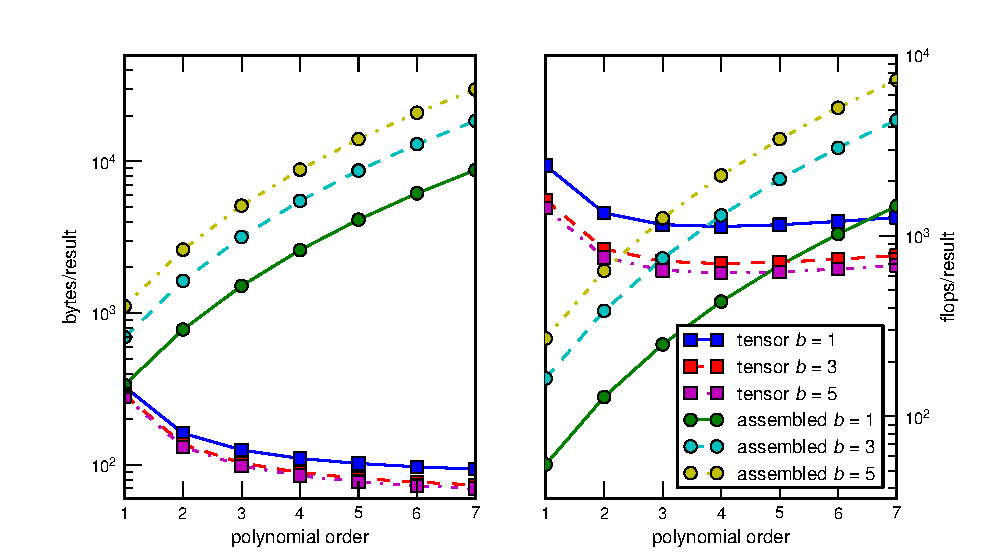
\includegraphics[width=\textwidth]{figures/TensorVsAssembly} \\
  \begin{itemize}
  \item High order Jacobian stored unassembled using coefficients at quadrature points, can use local AD
  \item Choose approximation order at run-time, independent for each field
  \item Precondition high order using assembled lowest order method
  \item Implementation $> 70\%$ of FPU peak, SpMV bandwidth wall $< 4\%$
  \end{itemize}
\end{frame}


\begin{frame}{$\tau$ formulation of Full Approximation Scheme (FAS)}
  \begin{itemize}
  \item classical formulation: ``coarse grid \emph{accelerates} fine grid $\searrow \nearrow$
  \item $\tau$ formulation: ``fine grid feeds back into coarse grid'' $\nearrow \searrow$
  \item To solve $N u = f$, recursively apply
    \begin{equation*}
      \begin{split}
        \text{pre-smooth} \:\: & \quad \tilde u^h \gets S^h_{\text{pre}}(u^h_0, f^h) \\
        \text{solve coarse problem for $u^H$} \:\: & \quad N^H u^H = \underbrace{I_h^H f^h}_{f^H} + \underbrace{N^H \hat I_h^H \tilde u^h - I_h^H N^h \tilde u^h}_{\tau_h^H} \\
        \text{correction and post-smooth} \:\: & \quad u^h \gets S^h_{\text{post}} \Big( \tilde u^h + I_H^h (u^H - \hat I_h^H \tilde u^h), f^h \Big) \\
      \end{split}
    \end{equation*}
    \begin{tabular}{llll}
      \toprule
      $I_h^H$ & residual restriction & $\hat I_h^H$ & solution restriction \\
      $I_H^h$ & solution interpolation & $f^H = I_h^H f^h$ & restricted forcing \\
      $\{S^h_{\text{pre}},S^h_{\text{post}}\}$ & \multicolumn{3}{l}{smoothing operations on the fine grid} \\
      \bottomrule
    \end{tabular}
  \item At convergence, $u^{H*} = \hat I_h^H u^{h*}$ solves the $\tau$-corrected coarse grid equation
    $N^H u^H = f^H + \tau_h^H$,
    thus $\tau_h^H$ is the ``fine grid feedback'' that makes the coarse grid equation accurate.
  \item $\tau_h^H$ is \emph{local} and need only be recomputed where it becomes stale.
  \end{itemize}
\end{frame}

\newcommand{\mglevelfine}{\ensuremath{\mglevel_{\mathrm{fine}}}}
\newcommand{\mglevel}{\ensuremath{\ell}}
\newcommand{\mglevelcp}{\ensuremath{\mglevel_{\mathrm{cp}}}}
\newcommand\mgdx{2.1em}
\newcommand\mgdy{2.2em}
\newcommand\mgloc[4]{(#1 + #4*\mgdx*#3,#2 + \mgdy*#3)}
\begin{frame}{Multiscale compression and recovery using $\tau$}
  \begin{tikzpicture}
    [scale=0.7,every node/.style={scale=0.7},
    >=stealth,
    restrict/.style={thick,double},
    prolong/.style={thick,double},
    cprestrict/.style={green!50!black,thick,double,dashed},
    control/.style={rectangle,red!40!black,draw=red!40!black,thick},
    mglevel/.style={rounded rectangle,draw=blue!50!black,fill=blue!20,thick,minimum size=6mm},
    checkpoint/.style={rectangle,draw=green!50!black,fill=green!20,thick,minimum size=6mm},
    mglevelhide/.style={rounded rectangle,draw=gray!50!black,fill=gray!20,thick,minimum size=6mm},
    tau/.style={text=red!50!black,draw=red!50!black,fill=red!10,inner sep=1pt},
    crelax/.style={text=green!50!black,fill=green!10,inner sep=0pt}
    ]
    \begin{scope}
      \node[mglevel] (fine0) at \mgloc{0}{0}{4}{-1} {\mglevelfine};
      \node[mglevel] (finem1down0) at \mgloc{0}{0}{3}{-1} {};
      \node[mglevel] (cp1down0) at \mgloc{0}{0}{2}{-1} {$\mglevelcp+1$};
      \node[mglevel] (cpdown0) at \mgloc{0}{0}{1}{-1} {\mglevelcp};
      \node[mglevel] (coarser0) at \mgloc{0}{0}{0}{0} {\ldots};

      \node[mglevelhide] (cpup0) at \mgloc{0}{0}{1}{1} {};
      \node (cp1up0) at \mgloc{0}{0}{2}{1} {};

      \node (cpdown1) at \mgloc{4em}{0}{1}{-1} {};
      \node[mglevelhide] (coarser1) at \mgloc{4em}{0}{0}{1} {\ldots};
      \node[mglevel] (cpup1) at \mgloc{4em}{0}{1}{1} {\mglevelcp};
      \node[mglevel] (cp1up1) at \mgloc{4em}{0}{2}{1} {$\mglevelcp+1$};
      \node[mglevel] (finem1up1) at \mgloc{4em}{0}{3}{1} {};
      \node[mglevel] (fine1) at \mgloc{4em}{0}{4}{1} {\mglevelfine};

      \draw[->,restrict,dashed] (fine0) -- (finem1down0);
      \draw[->,restrict] (finem1down0) -- (cp1down0);
      \draw[->,restrict] (cp1down0) -- (cpdown0);
      \draw[->,restrict,dashed] (cpdown0) -- (coarser0);
      \draw[->,prolong,dashed] (coarser0) -- (cpup0);
      \draw[->,prolong,dashed] (cpup0) -- (cp1up0);

      \draw[->,restrict,dashed] (cpdown1) -- (coarser1);
      \draw[->,prolong,dashed] (coarser1) -- (cpup1);
      \draw[->,prolong] (cpup1) -- (cp1up1);
      \draw[->,prolong] (cp1up1) -- (finem1up1);
      \draw[->,prolong,dashed] (finem1up1) -- (fine1);

      \node[checkpoint] at (4em + \mgdx*4,\mgdy) (cp) {CP};
      \draw[>->,cprestrict] (fine1) -- node[below,sloped] {Restrict} (cp);

      \node[left=\mgdx of fine0] (bnanchor) {};
      \node[control,fill=red!20] at (1.1*\mgdx,3*\mgdy) {Solve $F(u^n;b^n) = 0$};
      \node[mglevel,right=of fine1] (finedt) {next solve};
      \draw[->, >=stealth, control] (fine1) to[out=20,in=170] node[above] {$b^{n+1}(u^n,b^n)$} (finedt);
      \draw[->, >=stealth, control] (bnanchor) to[out=45,in=155] node[above] {$b^n$} (fine0);

      % Recovery process
      \begin{scope}[xshift=7.5*\mgdx]
        \node[checkpoint] (rcp) at \mgloc{0}{0}{0}{0} {CP};
        \node[mglevel] (r0a) at \mgloc{0}{\mgdy}{0}{0} {CR};
        \node[mglevel] (r1a) at \mgloc{0}{\mgdy}{1}{1} {};
        \node[mglevel] (r0b) at \mgloc{2*\mgdx}{\mgdy}{0}{0} {CR};
        \node[mglevel] (r1b) at \mgloc{2*\mgdx}{\mgdy}{1}{1} {};
        \node[mglevel] (r2b) at \mgloc{2*\mgdx}{\mgdy}{2}{1} {\mglevelfine};
        \node[mglevel] (r1c) at \mgloc{6*\mgdx}{\mgdy}{1}{-1} {};
        \node[mglevel] (r0d) at \mgloc{6*\mgdx}{\mgdy}{0}{0} {CR};
        \node[mglevel] (r1d) at \mgloc{6*\mgdx}{\mgdy}{1}{1} {};
        \node[mglevel] (r2d) at \mgloc{6*\mgdx}{\mgdy}{2}{1} {\mglevelfine};

        \draw[-,prolong,green!50!black] (rcp) -- (r0a);
        \draw[->,prolong] (r0a) -- (r1a);
        \draw[->,restrict] (r1a) -- (r0b);
        \draw[->,restrict] (r0b) -- (r1b);
        \draw[->,restrict,dashed] (r1b) -- (r2b);
        \draw[->,restrict,dashed] (r2b) -- (r1c);
        \draw[->,restrict] (r1c) -- (r0d);
        \draw[->,restrict] (r0d) -- (r1d);
        \draw[->,restrict,dashed] (r1d) -- (r2d);

        \foreach \smooth in {finem1down0, cp1down0, cpdown0, coarser0,
          cpup1, cp1up1, finem1up1,
          r0b,r1c,r0d,r1d} {
          \node[above left=-5pt of \smooth.west,tau] {$\tau$};
        }
        \node[rectangle,fill=none,draw=green!50!black,thick,fit=(rcp)(r2d)] (recoverbox) {};
        \node[rectangle,draw=green!50!black,fill=green!20,thick,minimum size=6mm,above={0cm of recoverbox.south east},anchor=south east] (recover) {FMG Decompression};
      \end{scope}
      \node (notation) at (2*\mgdx,5*\mgdy) {
        \begin{minipage}{18em}\small\sf
          \begin{itemize}\addtolength{\itemsep}{-5pt}
          \item checkpoint converged coarse state
          \item recover using FMG anchored at $\mglevelcp+1$
          \item needs only $\mglevelcp$ neighbor points
          \item $\tau$ correction is local
          \end{itemize}
        \end{minipage}
      };
    \end{scope}
  \end{tikzpicture}
  \vspace{-1em}
  \begin{itemize}
  \item Fine state $u^{h*}$ recovered \emph{locally} from converged coarse state $u^{H*} = \hat I_h^H u^{h*}$
  \item Normal multigrid cycles visit all levels moving from $n \to n+1$
  \item FMG recovery only accesses levels finer than $\ell_{CP}$
  \item Only need neighborhood of desired region for decompression
  \item Lightweight checkpointing for transient adjoint computation
  \item Postprocessing applications, e.g., in-situ visualization at high temporal resolution in part of the domain
  \end{itemize}
\end{frame}

\begin{frame}[shrink=5]{Four Schools of Thought for Multilevel Methods}
  \begin{itemize}
  \item Multigrid (Brandt, Hackbusch, $\dotsc$)
    \begin{itemize}
    \item originally for resolved/asymptotic spatial discretizations
    \item ``textbook'': reach discretization error in one F-cycle
    \item matrix-light/free, good for memory bandwidth
    \item FAS well-developed for nonlinear problems
    \end{itemize}
  \item Multilevel Domain Decomposition (Mandel, Dohrmann, Widlund)
    \begin{itemize}
    \item leverage direct subdomain solvers, minimize communication
    \item rapid coarsening $\kappa(P^{-1}A) \sim \big(1 + \log \frac H h \big)^{2(L-1)}$
    \item often formulated only as two-level methods, domain-conforming coefficients
    \item lightly developed for nonlinear (e.g. ASPIN [Cai and Keyes])
    \end{itemize}
  \item Multiscale Finite Elements (Babuska, Arbogast, $\dotsc$)
    \begin{itemize}
    \item local preprocessing to construct linear coarse operator
    \item popular in porous media and composite materials (robust theory)
    \end{itemize}
  \item Equation-based multiscale models (many)
    \begin{itemize}
    \item Renormalization multigrid/systematic upscaling (Brandt)
      \begin{itemize}
      \item interpolation, equilibriation (compatible relaxation/Monte-Carlo), restriction
      \end{itemize}
    \item Heterogeneous multiscale method (E, Engquist)
      \begin{itemize}
      \item reconstruction, constrained microscale simulation, data processing/compression
      \end{itemize}
    \end{itemize}
  \end{itemize}
\end{frame}


% Coarsening
\begin{frame}{Computable Convergence Measures (Linear correction notation)}
\newcommand\Vcoarse{V_{\text{coarse}}}
\newcommand\Vfine{V_{\text{fine}}}
  \begin{itemize}
  \item Prolongation $P: \Vcoarse \to \Vfine$
  \item Restriction $R: \Vfine \to \Vcoarse$
  \item Smoother $S^{-1} : \Vfine \to \Vfine$ should remove high-frequency component of error
  \item $I - PR: \Vfine \to \Vfine$ removes part of vector visible in coarse space
  \item Error iteration $I - M^{-1}A$, worst-case convergence factor is $\lambda_{\max}$
  \item ``Interpolation must be able to approximate an eigenvector with error bound proportional to the size of the associated eigenvalue.''
    \begin{itemize}
    \item Upper bound for convergence rate: $\max_x \norm{x}_{(I-PR)S(I-PR)}/{\norm{x}_A}$
    \end{itemize}
  \item Distinct challenges to constructing coarse space and operator
    \begin{itemize}
    \item Is the coarse space large enough to distinguish all low-energy modes?
    \item Are those modes accurately represented? (Is $P$ accurate enough?)
    \item Is the coarse operator accurate? (Automatic with Galerkin-type $RAP$ for nice problems.)
    \end{itemize}
  \end{itemize}
\end{frame}

\begin{frame}{Compatible Relaxation}
  \begin{columns}
    \begin{column}{0.5\textwidth}
      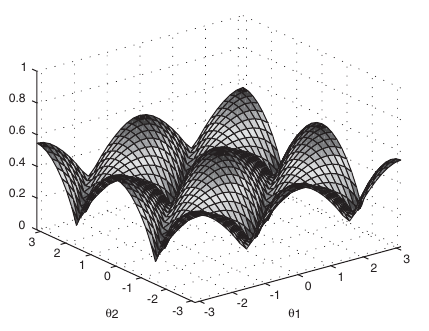
\includegraphics[width=\textwidth]{figures/LivneHabituatedCR} \\
      {\small [Livne 2004]}
    \end{column}
    \begin{column}{0.5\textwidth}
      \begin{itemize}
      \item Apply smoother subject to constraint $\hat R x = 0$
        \begin{enumerate}
        \item $\tilde x_n = x_{n-1} + S_A^{-1}\big(r(x_{n-1}) \big)$
        \item $x_n = \tilde x_n + S_R^{-1}\big(\hat R\tilde x_n) \big)$
        \end{enumerate}
      \item Method to determine when coarse space is rich enough
      \item Slow to relax points/regions good candidates for coarse points/aggregates
      \item If subdomain solves used for smoothing, only interfaces are candidates
      \end{itemize}
    \end{column}
  \end{columns}
\end{frame}

\begin{frame}{Coarse basis functions}
  \begin{itemize}
  \item $\norm{PR x}_A + \norm{(I - PR)x}_A \le C \norm{x}_A$
  \item ``decompose any $x$ into parts without increasing energy much''
  \item near-null spaces must be represented exactly (partition of unity)
  \item number of rows of $R$ determined already, usually $P = R^T$
  \item energy minimization with specified support [Wan, Chan, Smith; Mandel, Brezina, Vanek; Xu, Zikatanov]
  \item smoothed aggregation: $P_{\text{smooth}} = (I - \omega D^{-1} A) P_{\text{agg}}$
  \item classical AMG: each fine point processed independently
  \item domain decomposition/multiscale FEM: solve subdomain problems
  \end{itemize}
\end{frame}

\begin{frame}{Example: BDDC/FETI-DP coarse basis function}
    \begin{columns}
    \begin{column}{0.6\textwidth}
      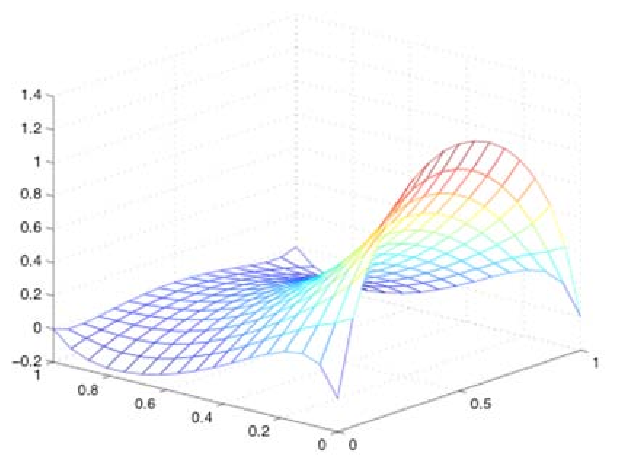
\includegraphics[width=\textwidth]{figures/MandelSousedikBDDCCoarseBasis} \\
      {\small [Mandel and Sousedik 2010]}
    \end{column}
    \begin{column}{0.4\textwidth}
      \begin{itemize}
      \item only low-order continuity between subdomains
      \item corrected by more technical subdomain smoother
      \end{itemize}
    \end{column}
  \end{columns}
\end{frame}

\begin{frame}{Why I like subdomain problems}
  \begin{columns}
    \begin{column}{0.4\textwidth}
      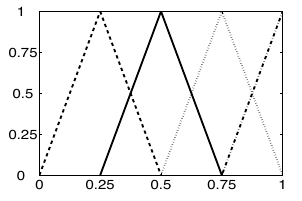
\includegraphics[width=\textwidth]{figures/ArbogastCoarse} \\
      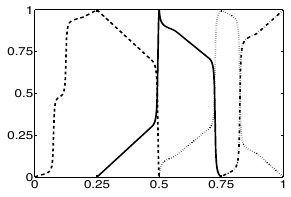
\includegraphics[width=\textwidth]{figures/ArbogastCoarseMs} \\
      {\small [Arbogast 2011]}
    \end{column}
    \begin{column}{0.6\textwidth}
      \begin{itemize}
      \item subassembly avoids explicit matrix triple product $A_{\text{coarse}} \gets P^T A_{\text{fine}} P$
      \item can update the coarse operator locally (e.g.~local nonlinearity)
      \item need not assemble entire fine grid operator
      \item if repetitive structure, need not store entire fine grid state
      \item can coarsen very rapidly (especially in smooth regions)
      \item lower communication setup phase
      \end{itemize}      
    \end{column}
  \end{columns}
\end{frame}

\begin{frame}{Subdomain Interfaces and Energy Minimization}
    \begin{columns}
    \begin{column}{0.5\textwidth}
      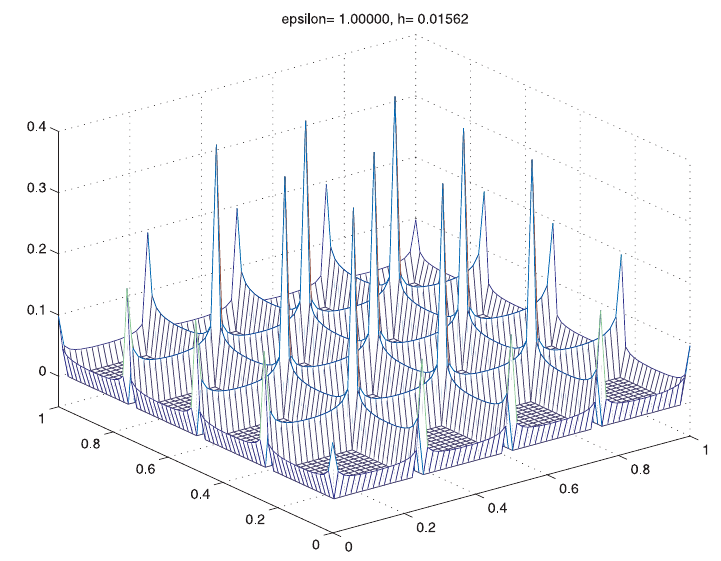
\includegraphics[width=\textwidth]{figures/MG/XuZikatanovLambda} \\
      {\small [Xu and Zikatanov 2004]}
    \end{column}
    \begin{column}{0.5\textwidth}
      \begin{itemize}
      \item minimize energy of all basis functions (columns of $P$) subject to
        \begin{itemize}
        \item fixed compact support
        \item partition of unity (near-null space)
        \end{itemize}
      \item enforce partition of unity using Lagrange multipliers
        \begin{itemize}
        \item $\lambda(x) = 0$ in coarse element interiors
        \item means that globally optimal coarse basis functions are harmonic extensions of \emph{some} interface values
        \end{itemize}
      \end{itemize}
    \end{column}
  \end{columns}
\end{frame}

\begin{frame}{Local edge/face-centered problems}
  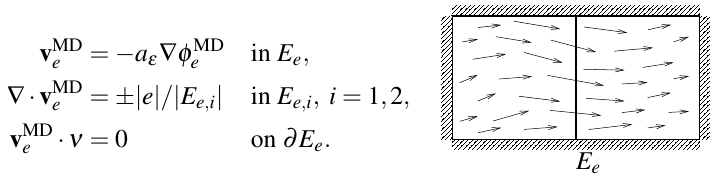
\includegraphics[width=0.9\textwidth]{figures/MG/ArbogastMultiscaleDual}
  \begin{itemize}
  \item Arbogast's multiscale dual-support elements for porous media
    \begin{itemize}
    \item inconsistent for unaligned anisotropy
    \item homogenization approach: upscale effective conductivity tensor from solution of periodic dual-support problem
    \end{itemize}
  \item Dohrmann and Pechstein's balancing domain decomposition for elasticity with unaligned coefficients
    \begin{itemize}
    \item balance ``torn'' interface values $u_{ie},u_{je}$, written in terms of subdomain Schur complements
    \item $\bar f_e = S_{iee} u_{ie} + S_{jee} u_{je}$: sum of forces required along face $e$ to displace subdomains $i$ and $j$ by $u_{ie}, u_{je}$
    \item $\bar u_e = (S_{iee} + S_{jee})^{-1} \bar f_e$: continuous displacement
    \item equivalent to a (different) dual-support basis
    \end{itemize}
  \end{itemize}
\end{frame}

\begin{frame}{Complication for saddle point problems}
  \begin{columns}
    \begin{column}{0.2\textwidth}
      \[ \begin{pmatrix}
        A & B^T \\ B & 0
      \end{pmatrix} \]
    \end{column}
    \begin{column}{0.8\textwidth}
      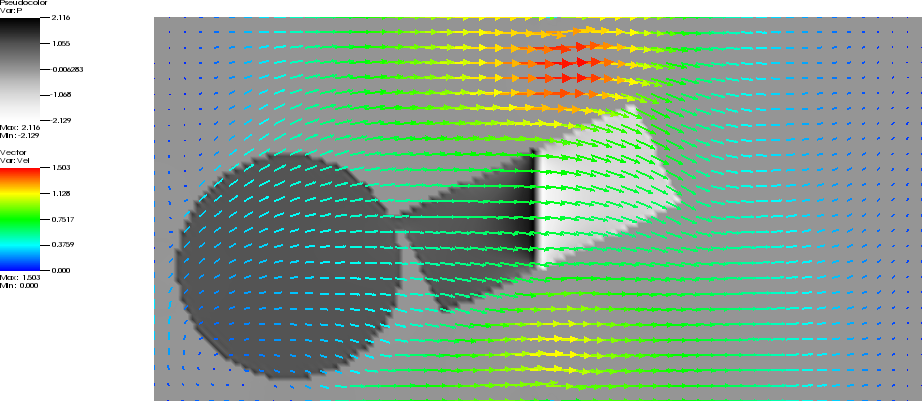
\includegraphics[width=\textwidth]{figures/MG/StokesDualProblem}
    \end{column}
  \end{columns}
  \begin{itemize}
  \item want uniform stability for coarse problem
    \begin{itemize}
    \item respect inf-sup condition, similar to fine grid
    \item make coarse grid mimic fine grid ($Q_2-P_1^{\text{disc}}$)
    \end{itemize}
  \item \emph{exact} representation of volumetric mode
    \begin{itemize}
    \item we can't cheat on conservation while upscaling
    \item naturally involves face integrals (inconvenient for recursive application)
    \item obtain similar quantity through solution of inhomogeneous Stokes problems
    \end{itemize}
  \item heuristic algebraic coarsening also possible [Adams 2004]
  \end{itemize}
\end{frame}


% Smoothing
\begin{frame}{Nonlinear problems}
  \begin{itemize}
  \item matrix-based smoothers require global linearization
  \item nonlinearity often more efficiently resolved locally
  \item nonlinear additive or multiplicative Schwarz
  \item nonlinear/matrix-free is good if
    \[ C = \frac{(\text{cost to evaluate residual at one point}) \cdot N}{(\text{cost of global residual})} \sim 1 \]
    \begin{itemize}
    \item finite difference: $C < 2$
    \item finite volume: $C \sim 2$, depends on reconstruction
    \item finite element: $C \sim \text{number of vertices per cell}$
    \end{itemize}
  \item larger block smoothers help reduce $C$
  \end{itemize}
  \vspace{-2.5em}
  \hfill 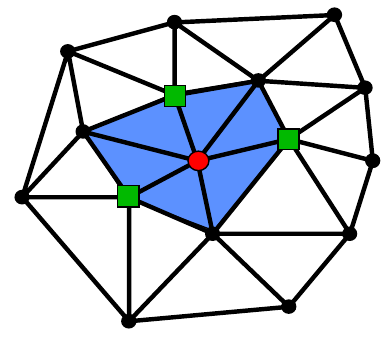
\includegraphics[width=0.3\textwidth]{figures/NodeStencil}
\end{frame}

\begin{frame}{Smoothing for saddle point systems}
  \begin{equation*}
  \begin{pmatrix}
    A & B^T \\ B & 0
  \end{pmatrix}
  \begin{pmatrix}
    u \\ p
  \end{pmatrix}
  =
  \begin{pmatrix}
    b \\ 0
  \end{pmatrix}
\end{equation*}
  \begin{itemize}
  \item pressure has no self-coupling
  \item pressure error modes not spectrally separated
  \item approaches
    \begin{itemize}
    \item block smoothers (Vanka)
    \item amplify fine-grid modes (distributive relaxation)
    \item splitting with approximate Schur complement
    \end{itemize}
  \end{itemize}
\end{frame}

\begin{frame}{Vanka block smoothers}
  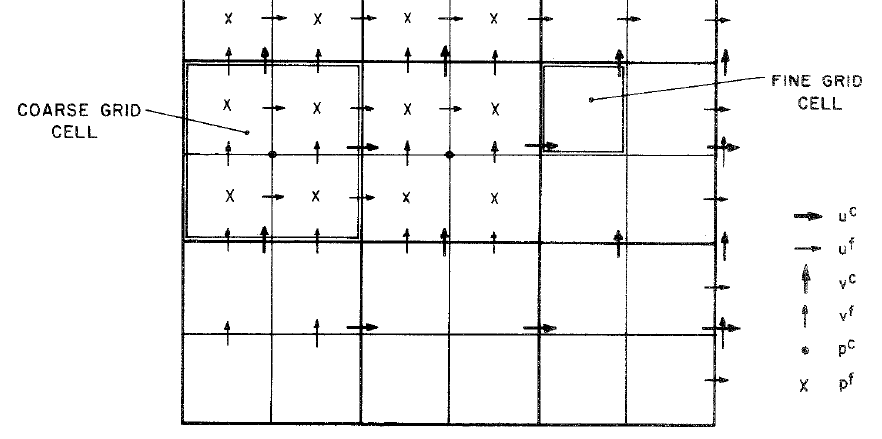
\includegraphics[width=0.9\textwidth]{figures/VankaStaggeredGrid} \\
  \begin{itemize}
  \item solve pressure-centered cell problems \\
    \quad (better for discontinuous pressure)
  \item robust convergence factor $\sim 0.3$ \emph{if} coarse grids are accurate
  \item 1D energy minimizing interpolants easy and effective
  \item can use assembled sparse matrices, but more efficient without
  \end{itemize}
\end{frame}

\begin{frame}{Changing Associativity: Distributive Smoothing}
  \begin{align*}
    P A x &= P b & AP y = b, & \quad x = Py
  \end{align*}
  \begin{itemize}
  \item Normal Preconditioning: make $PA$ or $AP$ well-conditioned
  \item Alternative: amplify high-frequency modes
    \begin{itemize}
    \item Multigrid smoothers only need to relax high-frequency modes
    \item Easier to do when spectrally separated: $h$-ellipticity
      \begin{itemize}
      \item pointwise smoothers (Gauss-Seidel) and polynomial/multistage methods
      \end{itemize}
    \item Mechanics: form the product $PA$ or $AP$ and apply ``normal'' method
    \item Example (Stokes)
      \begin{align*}
        A &\sim \begin{pmatrix} -\nabla^2 & -\nabla \\ \nabla\cdot &
          0 \end{pmatrix} &
        P &\sim \begin{pmatrix} \bm 1 & -\nabla \\ 0 & -\nabla^2 \end{pmatrix} &
        AP &\sim
        \begin{pmatrix}
          -\nabla^2 & \text{``0''} \\ \nabla\cdot & -\nabla^2
        \end{pmatrix}
      \end{align*}
    \end{itemize}
  \end{itemize}
\end{frame}

\begin{frame}[fragile]{Coupled MG for Stokes, split smoothers}
\begin{columns}
  \begin{column}{0.3\textwidth}
    \begin{align*}
      J &=
      \begin{pmatrix}
        A & B^T \\ B & C
      \end{pmatrix} \\
      P_{\text{smooth}} &=
      \begin{pmatrix}
        A_{\text{SOR}} & 0 \\
        B & M
      \end{pmatrix}
    \end{align*}
  \end{column}
  \begin{column}{0.7\textwidth}
    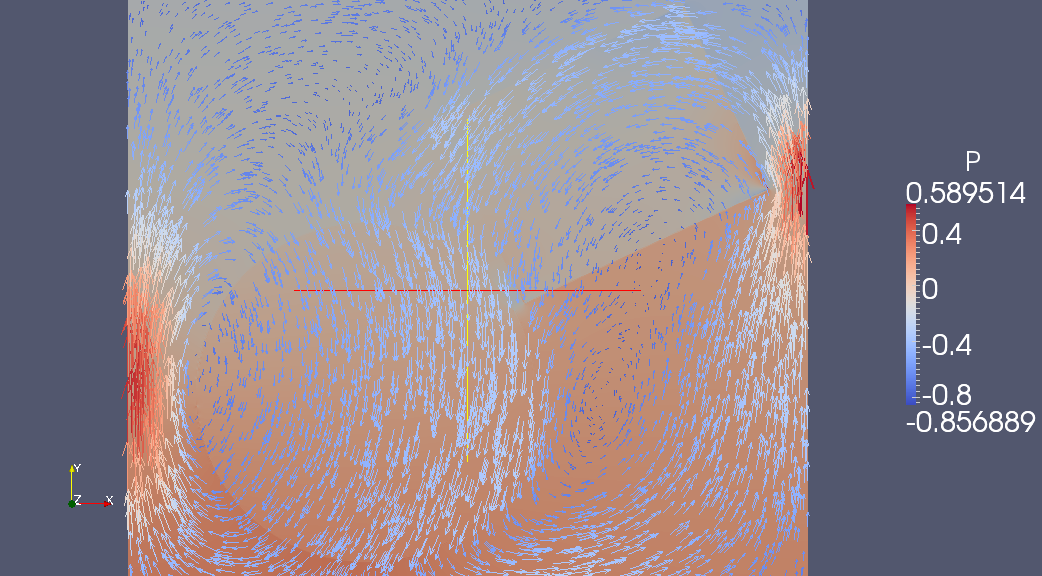
\includegraphics[width=\textwidth]{figures/Sinker2}
  \end{column}
\end{columns}
\begin{Verbatim}[formatcom=\footnotesize]
-pc_type mg -pc_mg_levels 5 -pc_mg_galerkin
-mg_levels_pc_type fieldsplit
-mg_levels_pc_fieldsplit_block_size 3
-mg_levels_pc_fieldsplit_0_fields 0,1
-mg_levels_pc_fieldsplit_1_fields 2
-mg_levels_fieldsplit_0_pc_type sor
\end{Verbatim}
\end{frame}


\begin{frame}{Outlook}
  \begin{itemize}
  \item smoothing with point-block Jacobi Chebyshev and scaled diagonal for pressure
  \item needs only (subdomain ``Neumann'') nonlinear function evaluations and assembly of point-block diagonal matrices
  \item convergence rates similar to smoothed aggregation, but without fine-grid assembly
  \item allows local updates of coarse operator, but currently slower due to naive implementation
  \item Development in progress within PETSc
    \begin{itemize}
    \item parallel implementation of dual-support problems without duplicating lots of work
    \item homogenization-based nonlinear coarsening
    \item true $\tau$ formulation with adaptive fine-grid visits and partial coarse operator updates
    \item microstructure-compatible pressure interpolation
    \item ``spectrally-correct'' nonlinear saddle-point smoothers
    \item locally-computable spectral estimates for guaranteed-stable additive smoothers
    \end{itemize}
  \end{itemize}
\end{frame}

\end{document}
